\section{Esposizione
dell\textquotesingle Architettura}\label{esposizione-dellarchitettura}

Sia \(k\in[0,\dots,n-1]\) con \(n\) il numero di team partecipenti.

La topologia e\textquotesingle{} suddivisa logicamente in più reti:

\begin{itemize}
\tightlist
\item
  \textbf{una rete di produzione per ogni team}, dove la rete
  \(\text{production-}k\) identifica gli oggetti di rete usati per
  collegare i container vulnerabili alla rete per il team \(k\)
\item
  \textbf{una o più reti di verifica, al più una per team}. la rete
  \(\text{verify-}k\) identifica gli oggetti di rete ed i container
  duplicati utilizzati per la verifica richiesta dal \(\text{team-}k\)
\end{itemize}

\subsection{\texorpdfstring{rete
\(\text{production-}k\)}{rete \textbackslash text\{production-\}k}}\label{rete-textproduction-k}

La rete \(\text{production-}k\) e\textquotesingle{} fatta cosi,
contiene:

\begin{itemize}
\tightlist
\item
  \(\text{wg-}k\): dispositivo L3, fa da terminazione per il tunnel del
  team \(k\) esimo. Assegna l\textquotesingle ip
  \passthrough{\lstinline!10.k.0.2/32!} al client che si collega.
\item
  \(\text{br-team-}k\): switch L2. Ha un gateway assegnato in modo da
  poter permettere all\textquotesingle Host di instradare da reti
  esterne.
\item
  \(\text{team-}k\text{-profile}\): profilo Incus per collegare
  l\textquotesingle interfaccia \(\text{eth}0\) del container del team
  \(k\) a \(\text{br-team-}k\)
\item
  \(\text{eth0}\): le interfacce di rete \(\text{eth0}\) dei container
  vengono collegate a \(\text{br-team-}k\).
\item
  regole per il forwarding e l\textquotesingle instradamento
  (\passthrough{\lstinline!nftables!}).
\end{itemize}


\begin{figure}[htbp]
  \centering
  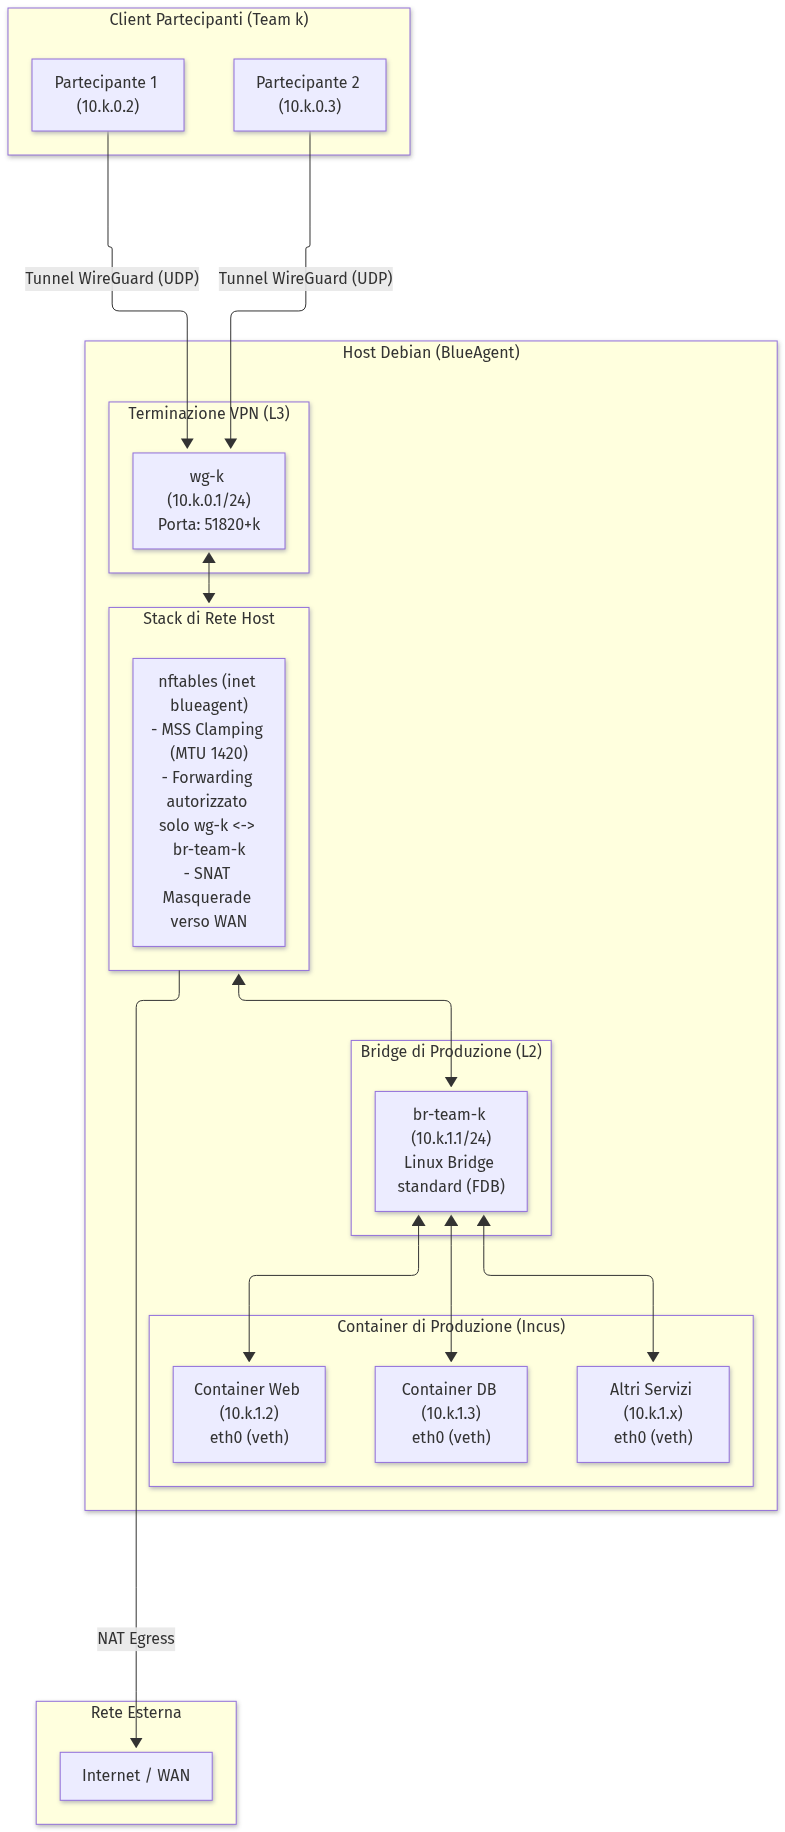
\includegraphics[width=0.92\linewidth,height=0.7\textheight,keepaspectratio]{src/images/mermaid_rete_production_k_ffe1d0312d.png}
  \caption{Rete Production K}
  \label{fig:mermaid_rete_production_k_ffe1d0312d}
\end{figure}


\begin{center}\rule{0.5\linewidth}{0.5pt}\end{center}

\subsection{\texorpdfstring{rete
\(\text{verify-}k\)}{rete \textbackslash text\{verify-\}k}}\label{rete-textverify-k}

La rete \(\text{verify-k}\) e\textquotesingle{} fatta cosi, contiene:

\begin{itemize}
\tightlist
\item
  \textbf{rete OVN} temporanea \(\text{verify-ovn-k}\). Implementa uno
  switch ed un router per instradare verso l\textquotesingle esterno
  utilizzando le regole NAT

  \begin{itemize}
  \tightlist
  \item
    ad \textbf{incus}: questa rete appare come un\textquotesingle unico
    oggetto di rete
  \item
    in \textbf{OVN}: abbiamo l\textquotesingle implementazione della
    rete \(\text{verify-ovn-}k\). Questa implementazione
    e\textquotesingle{} fatta di un router e di uno switch di rete open
    vswitch gestiti da OVN.
  \end{itemize}
\item
  \(\text{incusbr0}\): e\textquotesingle{} il bridge di rete di incus,
  qui passa il traffico che dalla rete ovn deve uscire verso
  l\textquotesingle esterno.
\item
  \(\text{eth0}\): le interfacce dei container instradano verso
  \(\text{verify-ovn-}k\). OVN si occupa di capire come instradare i
  pacchetti.
\item
  \textbf{container verificatore}:
  \passthrough{\lstinline!verify-runner-xxxx!} (IP
  \passthrough{\lstinline!10.k.1.250!}), istanza effimera che esegue gli
  script di verifica e gli exploit contro i target duplicati.
\end{itemize}


\begin{figure}[htbp]
  \centering
  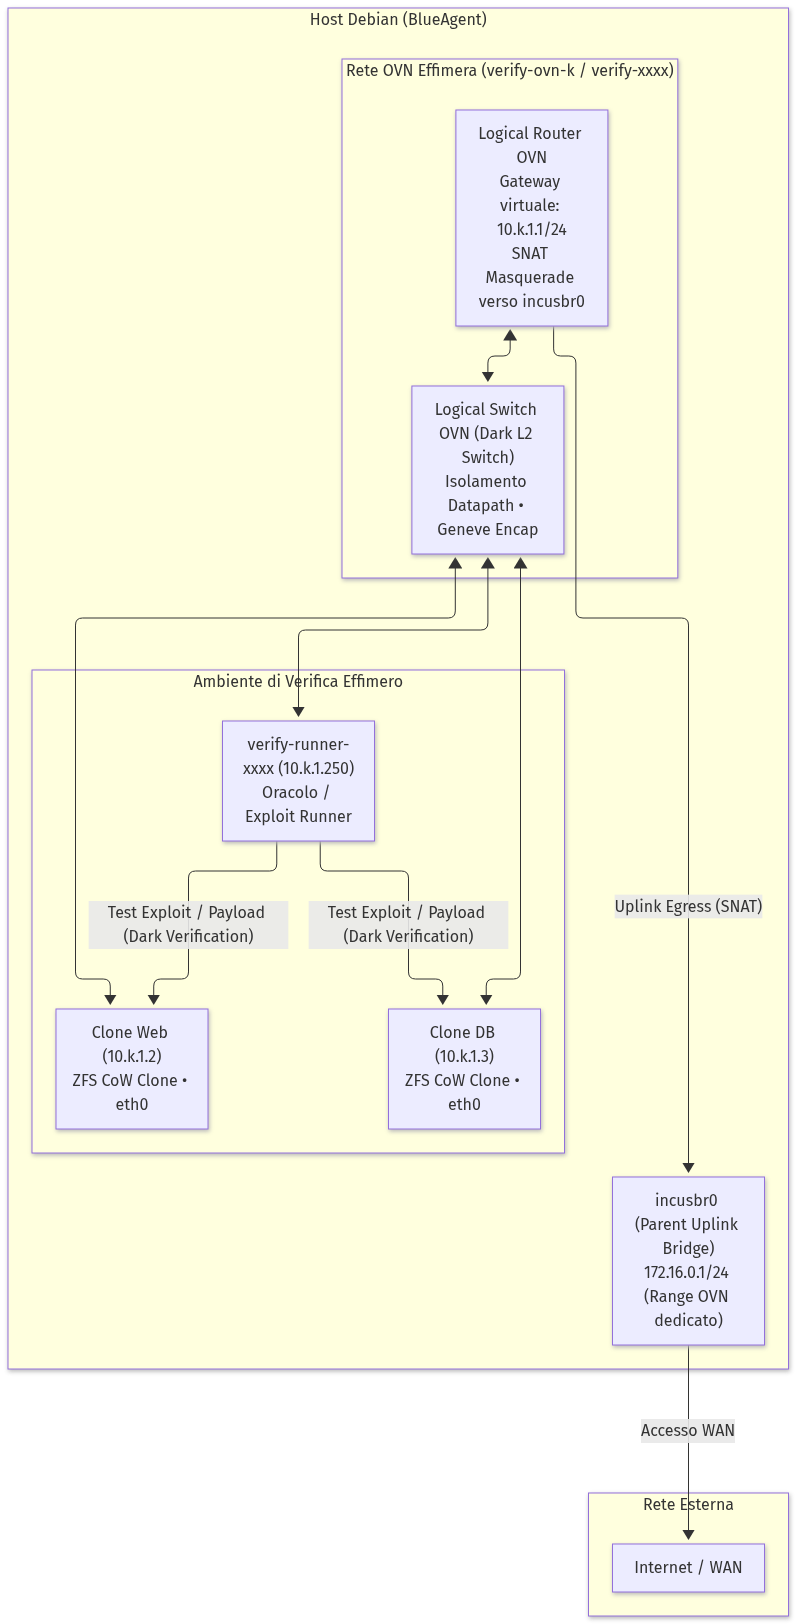
\includegraphics[width=0.92\linewidth,height=0.7\textheight,keepaspectratio]{src/images/mermaid_rete_verify_k_6657a97d3d.png}
  \caption{Rete Verify K}
  \label{fig:mermaid_rete_verify_k_6657a97d3d}
\end{figure}


\begin{center}\rule{0.5\linewidth}{0.5pt}\end{center}

\subsection{vista integrata (merge produzione e
verifica)}\label{vista-integrata-merge-produzione-e-verifica}

La coesistenza tra la rete di produzione e la sandbox di verifica su uno
stesso host fisico mette in risalto il principio di \textbf{fedeltà
topologica} e il \textbf{totale isolamento del traffico}:

\begin{enumerate}
\def\labelenumi{\arabic{enumi}.}
\tightlist
\item
  \textbf{Topologia e Indirizzamento Invarianti}: I container clonati
  mantengono esattamente lo stesso indirizzo IP statico
  (\passthrough{\lstinline!10.k.1.x!}) e lo stesso gateway
  (\passthrough{\lstinline!10.k.1.1/24!}) della produzione.
\item
  \textbf{Zero Conflitti di Routing sull\textquotesingle Host}:
  Sull\textquotesingle host esiste solo il gateway L3 di
  \passthrough{\lstinline!br-team-k!}. La rete
  \passthrough{\lstinline!verify-xxxx!} opera interamente
  all\textquotesingle interno del datapath di Open vSwitch/OVN senza
  creare interfacce L3 o rotte in conflitto nella tabella di routing del
  kernel Linux.
\item
  \textbf{Isolamento Completo (Dark Verification)}: Il traffico di
  exploit inviato dal \passthrough{\lstinline!verify-runner!} è
  confinato allo switch virtuale OVN: non può essere intercettato su
  \passthrough{\lstinline!br-team-k!} o tramite
  \passthrough{\lstinline!tcpdump!} dai partecipanti, e un eventuale
  crash distruttivo non ha ripercussioni sui container live.
\end{enumerate}


\begin{figure}[htbp]
  \centering
  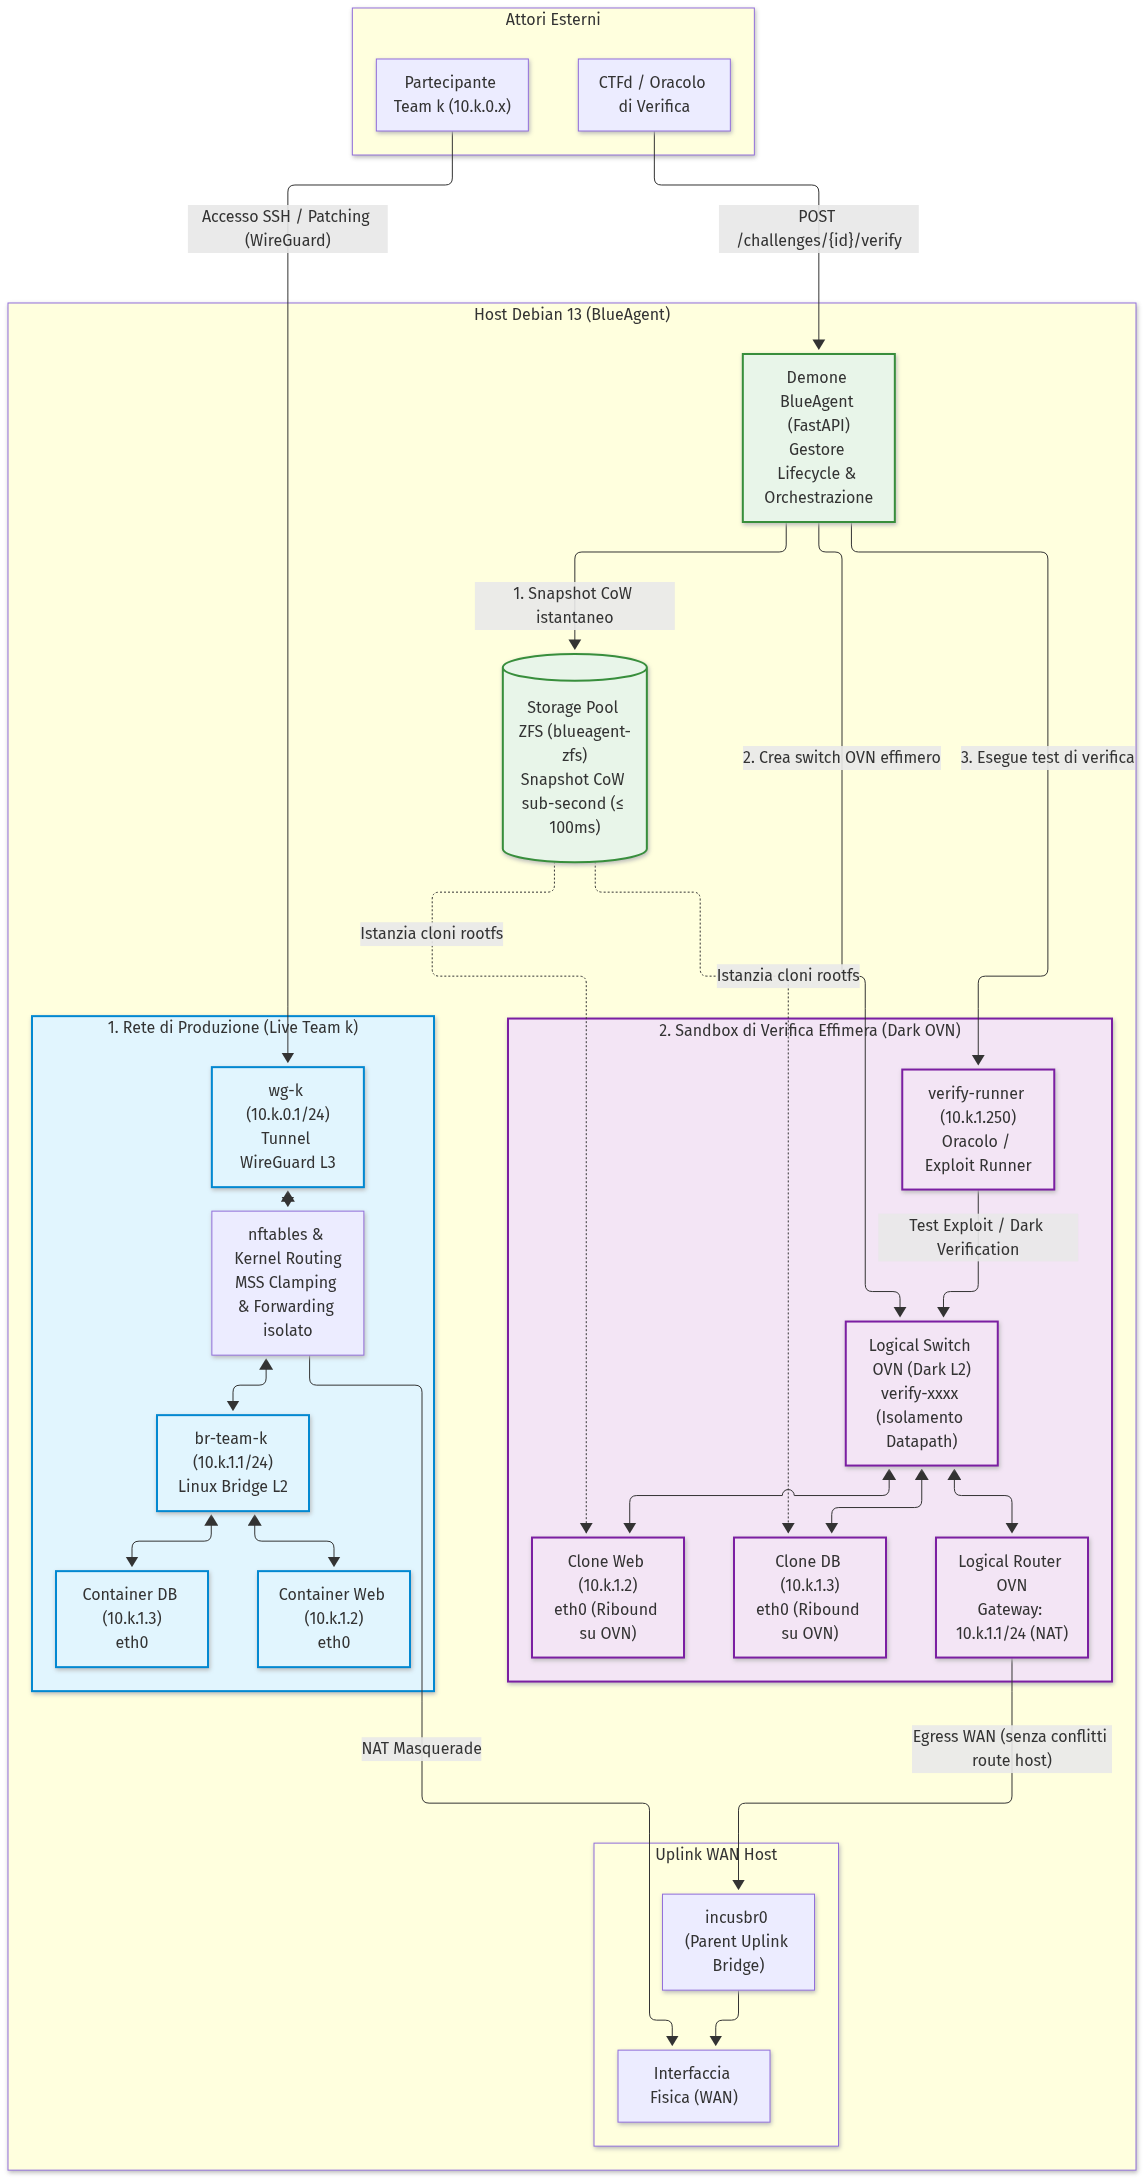
\includegraphics[width=0.92\linewidth,height=0.7\textheight,keepaspectratio]{src/images/mermaid_vista_integrata_merge_produzione_e_verifica_8073cbc52d.png}
  \caption{Vista Integrata Merge Produzione E Verifica}
  \label{fig:mermaid_vista_integrata_merge_produzione_e_verifica_8073cbc52d}
\end{figure}

